\section{CMOS Transistors and Logic}

\begin{frame}{Transistors}
	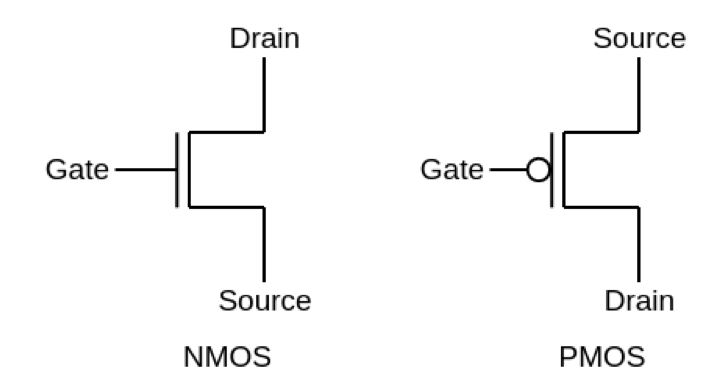
\includegraphics[width=0.5\textwidth]{./images/mos.png}
	    
	Two varieties of MOSFETs: P-type and N-type
	\\
	Any MOSFET has a characteristic threshold voltage $V_{th}$
	\\
	NMOS "turns on" (connects drain to source) when $V_{GS}>V_{th}$
	\\
	PMOS turns on when $V_{GS}<V_{th}$
\end{frame}
	
\begin{frame}{NMOS Logic}
	We can build an inverter (a circuit that flips a 1 to a 0 and vice versa) with a single N-type MOSFET! \\
	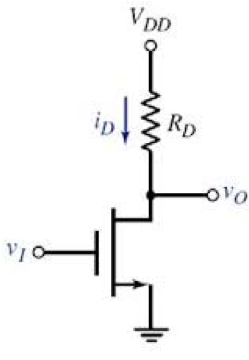
\includegraphics[width=0.2\textwidth]{./images/nmos-inverter.png}
	\\
	What is $v_O$ when $v_I>V_{th}$? When $v_I<V_{th}$?
	\\
	Key disadvantage: what is the power dissipated when $v_I>V_{th}$? How can we rectify this?
\end{frame}

\begin{frame}{CMOS Logic}
	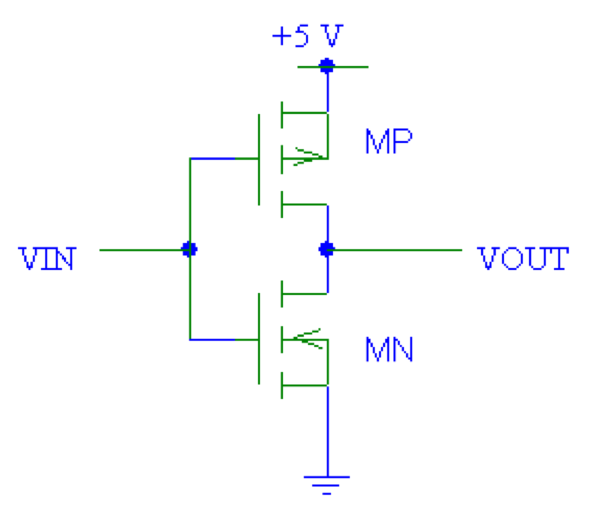
\includegraphics[width=0.4\textwidth]{./images/cmos-inverter.png}
	\\
	Now, we have the same logical function as the NMOS inverter, but we're using more transistors and much less power is dissipated. Why?
\end{frame}

\begin{frame}{CMOS Logic}
	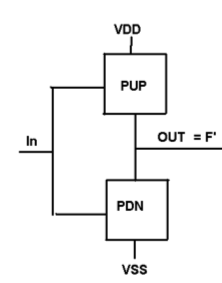
\includegraphics[width=0.3\textwidth]{./images/cmos.png}
	
	This is broadly called Complementary Metal Oxide Semiconductor (CMOS) logic, using a Pull-Up Network of P-type and a Pull-Down Network of N-type MOSFETs.
	\\
	Now we can build circuits that perform logical functions out of MOSFETs!
\end{frame}

\begin{frame}{Transistors \& CMOS Wrap-up}
	True or False:
	\begin{enumerate}
	    \item<1-> Power (in the EE16B model) is dissipated in a CMOS circuit only when there is switching \\
	    \onslide<2->{\textbf{True}}
	    \item<1-> NMOS devices turn on with a large VGS and off with low VGS \\
	    \onslide<3->{\textbf{True}}
        \item<1-> For a given choice of inputs in a CMOS inverter circuit, we can create a low resistance path from ground to high voltage \\
	    \onslide<4->{\textbf{False}}
	\end{enumerate}
\end{frame}
